\chapter{METODOLOGI}
Metodologi penelitian yang akan dilakukan di dalam penelitian ini adalah melalui pendekatan \textit{Design Science Research Methodology for Information Systems Research} (Peffers, et al, 2008)~\cite{geerts_design_2011}. Metodologi penelitian terdiri dari enam tahapan seperti digambarkan pada Gambar \ref{fig:dsrm} yaitu: identifikasi masalah dan motivasi, penentuan tujuan dari penelitian, perancangan dan pengembangan solusi/demonstrasi, pengujian dan pembahasan, pengambilan kesimpulan. Penelitian ini akan menggunakan strategi \textit{sequential exploratory design} yang akan dilakukan dalam dua tahap, tahap pertama dilakukan secara kualitatif, dan tahap kedua secara kuantitatif. Hasil temuan kualitatif pada tahap pertama, akan dilanjutkan dengan analisis kuantitatif pada tahap kedua.

\begin{figure}[H]
    \centering
    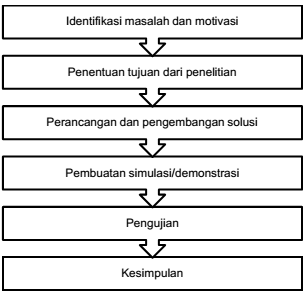
\includegraphics[height=6cm]{images/dsrm}
    \caption{Tahapan \textit{Design Science Research Methodology (DSRM)}}
    \label{fig:dsrm}
\end{figure}

Pada tahap pertama atau kualitatif, akan dilakukan studi literatur yang terkait dengan permasalahan penelitian, kemudian akan dikombinasikan dengan hasil pemeriksaan dokumen. Hal ini dilakukan untuk mengimplementasikan konsep triangulasi yaitu perbedaan sumber data dan metode pengumpulan data. Pada tahap kedua atau tahap kuantitatif, akan dilakukan pengujian terhadap variabel-variabel penelitian untuk menjelaskan hubungan antara variabel-variabel tersebut melalui pengujian hipotesis menggunakan metode statistik. Metode yang digunakan dalam pengumpulan data adalah metode survei dengan menghimpun persepsi responden mengenai variabel-variabel yang ditanyakan melalui instrumen berupa daftar pertanyaan berstruktur (kuesioner).
\begin{enumerate}
\item Identifikasi Masalah dan Motivasi

Pada tahapan ini melakukan identifikasi terhadap masalah yang ada, terutama berdasarkan teknologi dan kondisi yang ada. Identifikasi dilakukan dengan melakukan kajian untuk memahami dan menentukan motivasi berdasarkan hasil dari studi literatur. Studi dilakukan terhadap jurnal penelitian internasional, tesis, dan buku-buku teori pendukung nasional dan internasional. Peneliti melakukan analisis, interpretasi, dan generalisasi fakta-fakta dari literatur yang didapatkan. Studi juga dilakukan terhadap kondisi saat ini melalui pengumpulan data-data yang tersedia. Studi pustaka dilakukan untuk mendapatkan konsep dari fenomena yang terjadi. Dari fenomena dan konsep tersebut, kemudian dapat dirumuskan masalah, tujuan penelitian, batasan masalah dan pertanyaan penelitian.
\item Penentuan Fokus dari Penelitian

Penentuan fokus ditentukan berdasarkan hasil identifikasi masalah dan motivasi yang mendorong dilakukannya penelitian. Fokus penelitian adalah perancangan desain dan implementasi sistem terdistribusi pada perangkat mobile. Pembuatan proposal dilakukan sebagai pedoman dalam melakukan penelitian.
\item Perancangan dan Pengembangan Solusi

Perancangan dan pembuatan solusi berdasarkan fokus dari penelitian yaitu perancangan desain dan implementasi sistem terdistribusi pada perangkat mobile. Tahap pengembangan desain dilakukan dengan berbasis pada teori, yang terdiri dari tahap identifikasi masalah pada sistem terdistribusi berbasis perangkat mobile, kemudian perancangan desain sistem terdistribusi dan dilanjutkan dengan implementasi desain pada perangkat mobile. Tahap terakhir adalah pengujian desain serta model yang diteliti.
\item Pembuatan Simulasi / Demonstrasi

Berdasarkan rancangan solusi yang dibuat, pembuatan simulasi/demonstrasi dibangun dengan tujuan menguji rancangan solusi yang dibuat untuk melihat kesesuaian rancangan dengan harapan yang ingin dicapai.
\item Pengujian

Pengujian dilakukan untuk memastikan desain yang dirancang sesuai dengan kebutuhan sehingga dapat menyelesaikan permasalahan yang diangkat pada penelitian ini. Dalam penelitian, desain dan prototype diuji melalui beberapa skenario, antara lain : connection-full, connection-less, dan delay-based. Dalam pengujian, variable yang akan diukur antara lain : konsistensi, transparansi, waktu respon, dan trafik.
\item Analisis

Analisis dilakukan terhadap hasil pengujian yang didapatkan. Analisis bertujuan memberikan gambaran kondisi aplikasi dan masukan mengenai arah pengembangan lebih lanjut. Setelah data diolah, kemudian hasilnya dianalisis dan dibahas sesuai teori yang mendasari dan kriteria-kriteria pada model persamaan struktural. Hasil analisis harus dapat menjawab hipotesis yang ditentukan di awal penelitian. Selain itu, karena penelitian ini studi kasus, maka hasil dari perhitungan statistik dan berdasarkan teori maka dibuat pembahasan sesuai kontekstual tempat studi kasus. Dalam pembahasan diulas hasil penelitian ini dibandingkan dengan penelitianpenelitian sebelumnya.
\item Kesimpulan

Kesimpulan berdasarkan hasil dari tahapan penelitian yang telah dilakukan sebelumnya yang merupakan jawaban dari permasalahan serta perwujudan dari tujuan yang dicapai dari penelitian. Diharapkan hasil penelitian dapat memberikan kontribusi dalam mengatasi permasalahan yang ada.
\end{enumerate}

